\chapter{Comparing Objects}\label{sec:comp}

\section{Equivalence Relations}

Mathematicians have some precise words to say whether something is identical to, indistinguishable from, or just for all intents and purposes equivalent to something else.  So let's go over those words.

\begin{definition}[Equivalence Relation]
  An \textbf{Equivalence Relation} $ \sim $ is a property between two objects that is
  \begin{enumerate}
    \item \textbf{Reflexive} $a \sim a$
    \item \textbf{Symmetric} $a \sim b \rightarrow b \sim a$
    \item \textbf{Transitive} If $a\sim b$ and $b \sim c$ then $a \sim c$
  \end{enumerate}
\end{definition}

Say my equivalence relation is ``is the same color as".  Then
\begin{itemize}
  \item ocean $ \sim $ sky
  \item grass $ \sim $ trees
  \item sunburn $ \sim $ lobster
\end{itemize}

Or I could use an equivalence relation that is "could be deformed into without cutting, tearing, or gluing".  Then

\begin{tabular}{c c c}

\includegraphics[width=.4\textwidth,align=c]{pics/shawl.JPG} & {\fontsize{50}{60}\selectfont $\sim$} & 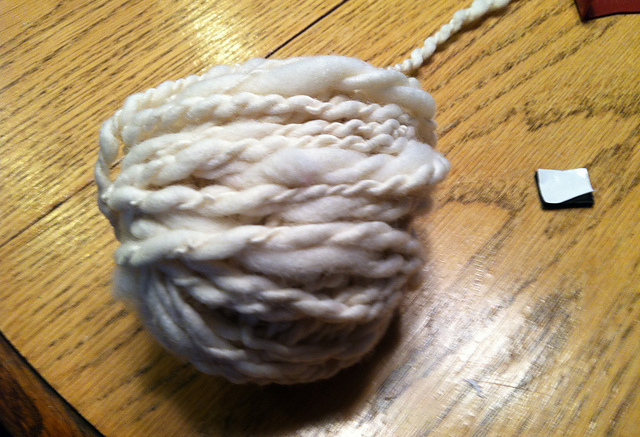
\includegraphics[width=.4\textwidth,align=c]{pics/yarn.JPG} \\
\end{tabular}

Let's treat these as ``ideal" objects, and forget about the fact the shawl is created from multiple different yarns, and that yarn itself is constructed from a vast number of individual fibers.


\begin{tabular}{c c c c c}
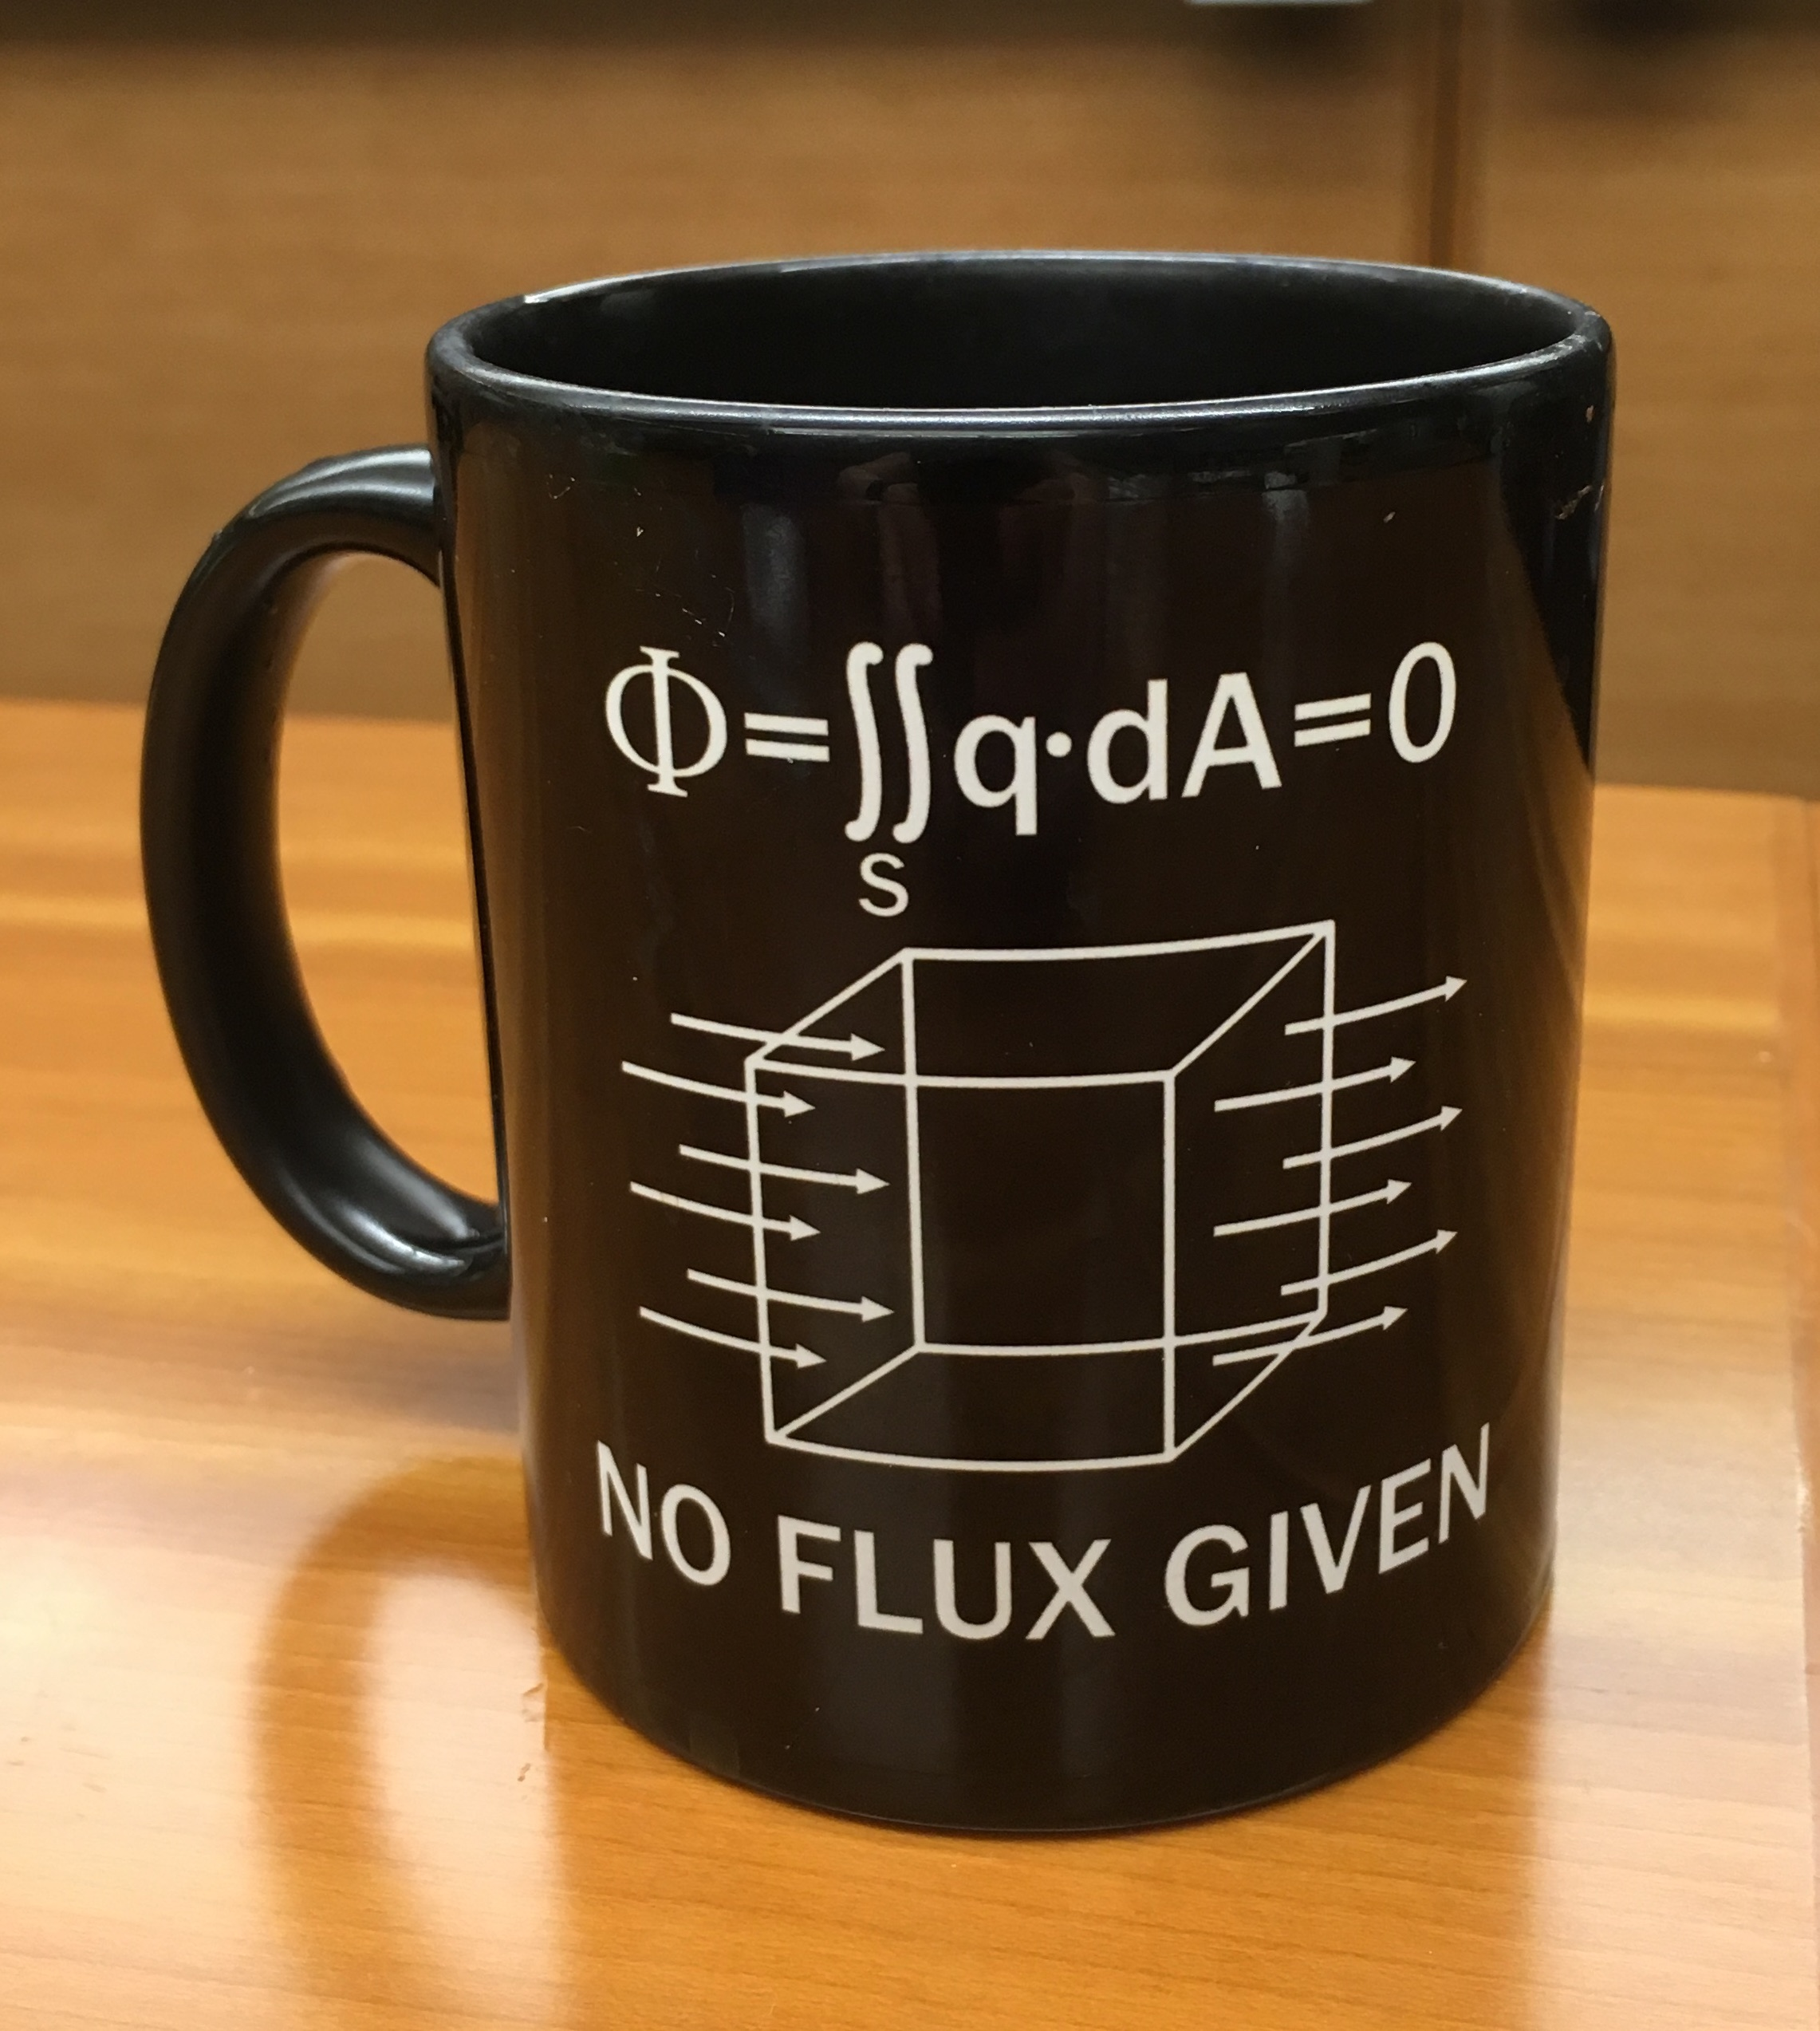
\includegraphics[width=.2\textwidth,align=c]{pics/mug.JPG} &
{\fontsize{50}{60}\selectfont $\sim$} &
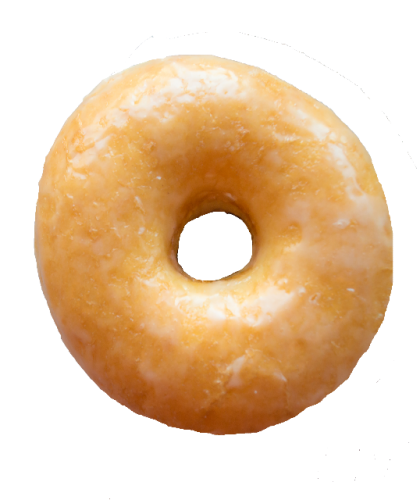
\includegraphics[width=.2\textwidth,align=c]{pics/donut.png}\protect\footnotemark &
{\fontsize{50}{60}\selectfont $\nsim$} &
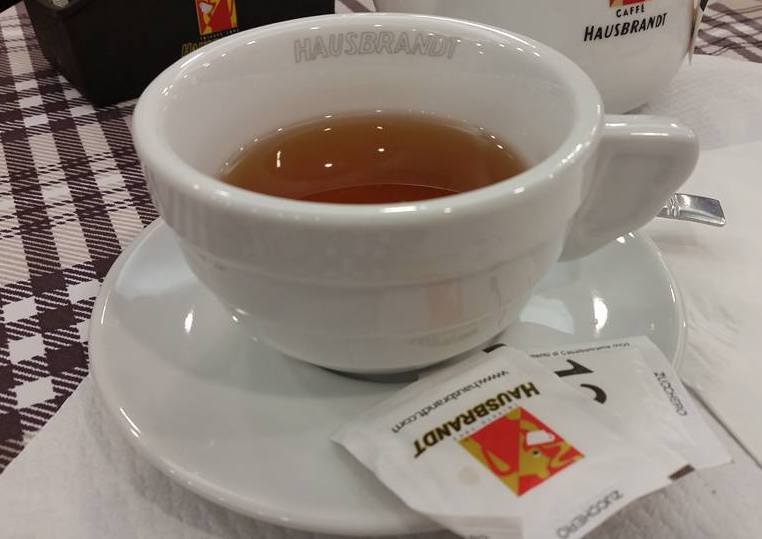
\includegraphics[width=.2\textwidth,align=c]{pics/not_a_donut.jpg} \\
\end{tabular}
\footnotetext{ http://pngimg.com/download/32474/?i=1}

\section{Equivalence Classes}

An equivalence relation can be used to define \textbf{equivalence classes}.

\begin{definition}[Equivalence Class]
  Given a set $S$ and a equivalence relation $\sim$ on elements in $S$, given an element $a\in S$, the \textbf{equivalence class} $[ a ] = \{ b \in S | b \sim a\}$.
\end{definition}

For $[a]$, $a$ is called the \textit{character} of that specific equivalence class, but we can use difference characters to represent the same equivalence class.  For example, if $a\sim b$, then $[a]$ and $[b]$ are the same thing.

An equivalence classes groups a bunch of things together based on similarity.  For example, we could use the equivalence relation "is same food group".  Then [apple] would represent all fruits.  I could equally write [orange] and mean the exact same thing.  But [croissant] would represent a different equivalence class, one that makes loaves of bread, tarts, scones, and muffins indistinguishable.

We do this all the time, even if we don't know it has the formal mathematical name of ``equivalence class''.  The term ``whales'' is just our way of grouping into a pile all humpbacks, blue whales, and right whales, given the equivalence relationship, "eats same way".  Well, maybe the relationship has a few more qualifiers.

Given a set and an equivalence relation, we can create a new set whose members are equivalence classes.  For example, let's say our initial set is everything on Earth, and the equivalence relation is ``is the same color as''.  We would end up with a set where one element was ``blue things'', another ``red things'', another ``green things''.  For the purposes of this explanation, let's simplify everything by saying objects will be either blue or green or some other nice pure color, not like those paint swatches you see at a hardware store with 150 shades of white.

For a math example, let the set be Integers $\mathbb{Z}$ and the equivalence relation be ``same parity''.  $1 \sim 3 \sim 5 \nsim 2$.  Now we have a new set with two elements, $[1]$ and $[2]$.

\section{Quotient Space}

\begin{definition}[Quotient Space]
  A \textbf{Quotient space} $S/\sim$ for a set $S$ and an equivalence relation $\sim$ is the set formed by equivalences classes in $S$ under $\sim$.
\end{definition}

Going back to the Integers $\mathbb{Z}$ and the equivalence relation ``same parity'', $\mathbb{Z}/ \sim  \approx \mathbb{Z}_2$.  I use $\approx$ as the answer isn't the group $\mathbb{Z}_2$, but just equivalent to $\mathbb{Z}_2$.  Instead, it's a group composed of the elements $[1]$ and $[2]$, where each element is an equivalence class.  This distinction might seem like a silly bit of finicky-ness here. When we are dealing with a set of loops, later on, I want you to remember that each member of the set is a geometric thing, or a collection of geometric things, though we map those objects onto numbers to be able to quantify and say things about them.




So far, these have been fun little real-world examples, but our equivalence relations can also divide materials up into similar phases, divide Hamiltonians up into groups with the same symmetries, or identify all wavefunctions equivalent up to a phase.
